\documentclass[twoside]{book}

% Packages required by doxygen
\usepackage{calc}
\usepackage{doxygen}
\usepackage{graphicx}
\usepackage[utf8]{inputenc}
\usepackage{makeidx}
\usepackage{multicol}
\usepackage{multirow}
\usepackage{textcomp}
\usepackage[table]{xcolor}

% Font selection
\usepackage[T1]{fontenc}
\usepackage{mathptmx}
\usepackage[scaled=.90]{helvet}
\usepackage{courier}
\usepackage{amssymb}
\usepackage{sectsty}
\renewcommand{\familydefault}{\sfdefault}
\allsectionsfont{%
  \fontseries{bc}\selectfont%
  \color{darkgray}%
}
\renewcommand{\DoxyLabelFont}{%
  \fontseries{bc}\selectfont%
  \color{darkgray}%
}

% Page & text layout
\usepackage{geometry}
\geometry{%
  a4paper,%
  top=2.5cm,%
  bottom=2.5cm,%
  left=2.5cm,%
  right=2.5cm%
}
\tolerance=750
\hfuzz=15pt
\hbadness=750
\setlength{\emergencystretch}{15pt}
\setlength{\parindent}{0cm}
\setlength{\parskip}{0.2cm}
\makeatletter
\renewcommand{\paragraph}{%
  \@startsection{paragraph}{4}{0ex}{-1.0ex}{1.0ex}{%
    \normalfont\normalsize\bfseries\SS@parafont%
  }%
}
\renewcommand{\subparagraph}{%
  \@startsection{subparagraph}{5}{0ex}{-1.0ex}{1.0ex}{%
    \normalfont\normalsize\bfseries\SS@subparafont%
  }%
}
\makeatother

% Headers & footers
\usepackage{fancyhdr}
\pagestyle{fancyplain}
\fancyhead[LE]{\fancyplain{}{\bfseries\thepage}}
\fancyhead[CE]{\fancyplain{}{}}
\fancyhead[RE]{\fancyplain{}{\bfseries\leftmark}}
\fancyhead[LO]{\fancyplain{}{\bfseries\rightmark}}
\fancyhead[CO]{\fancyplain{}{}}
\fancyhead[RO]{\fancyplain{}{\bfseries\thepage}}
\fancyfoot[LE]{\fancyplain{}{}}
\fancyfoot[CE]{\fancyplain{}{}}
\fancyfoot[RE]{\fancyplain{}{\bfseries\scriptsize Generated on Thu Mar 24 2016 16\-:45\-:49 for cs371p-\/allocator by Doxygen }}
\fancyfoot[LO]{\fancyplain{}{\bfseries\scriptsize Generated on Thu Mar 24 2016 16\-:45\-:49 for cs371p-\/allocator by Doxygen }}
\fancyfoot[CO]{\fancyplain{}{}}
\fancyfoot[RO]{\fancyplain{}{}}
\renewcommand{\footrulewidth}{0.4pt}
\renewcommand{\chaptermark}[1]{%
  \markboth{#1}{}%
}
\renewcommand{\sectionmark}[1]{%
  \markright{\thesection\ #1}%
}

% Indices & bibliography
\usepackage{natbib}
\usepackage[titles]{tocloft}
\setcounter{tocdepth}{3}
\setcounter{secnumdepth}{5}
\makeindex

% Hyperlinks (required, but should be loaded last)
\usepackage{ifpdf}
\ifpdf
  \usepackage[pdftex,pagebackref=true]{hyperref}
\else
  \usepackage[ps2pdf,pagebackref=true]{hyperref}
\fi
\hypersetup{%
  colorlinks=true,%
  linkcolor=blue,%
  citecolor=blue,%
  unicode%
}

% Custom commands
\newcommand{\clearemptydoublepage}{%
  \newpage{\pagestyle{empty}\cleardoublepage}%
}


%===== C O N T E N T S =====

\begin{document}

% Titlepage & ToC
\hypersetup{pageanchor=false}
\pagenumbering{roman}
\begin{titlepage}
\vspace*{7cm}
\begin{center}%
{\Large cs371p-\/allocator \\[1ex]\large 3 }\\
\vspace*{1cm}
{\large Generated by Doxygen 1.8.6}\\
\vspace*{0.5cm}
{\small Thu Mar 24 2016 16:45:49}\\
\end{center}
\end{titlepage}
\clearemptydoublepage
\tableofcontents
\clearemptydoublepage
\pagenumbering{arabic}
\hypersetup{pageanchor=true}

%--- Begin generated contents ---
\chapter{cs371p-\/allocator}
\label{md_README}
\hypertarget{md_README}{}
Estimated time for Completion\-: 8 hours

Nari Jeong (njv275)

Nishil Shah (nbs439) 
\chapter{Hierarchical Index}
\section{Class Hierarchy}
This inheritance list is sorted roughly, but not completely, alphabetically\-:\begin{DoxyCompactList}
\item \contentsline{section}{Allocator$<$ T, N $>$}{\pageref{classAllocator}}{}
\item Test\begin{DoxyCompactList}
\item \contentsline{section}{Test\-Allocator1$<$ A $>$}{\pageref{structTestAllocator1}}{}
\item \contentsline{section}{Test\-Allocator3$<$ A $>$}{\pageref{structTestAllocator3}}{}
\end{DoxyCompactList}
\end{DoxyCompactList}

\chapter{Class Index}
\section{Class List}
Here are the classes, structs, unions and interfaces with brief descriptions\-:\begin{DoxyCompactList}
\item\contentsline{section}{\hyperlink{classAllocator}{Allocator$<$ T, N $>$} }{\pageref{classAllocator}}{}
\item\contentsline{section}{\hyperlink{structTestAllocator1}{Test\-Allocator1$<$ A $>$} }{\pageref{structTestAllocator1}}{}
\item\contentsline{section}{\hyperlink{structTestAllocator3}{Test\-Allocator3$<$ A $>$} }{\pageref{structTestAllocator3}}{}
\end{DoxyCompactList}

\chapter{File Index}
\section{File List}
Here is a list of all files with brief descriptions\-:\begin{DoxyCompactList}
\item\contentsline{section}{\hyperlink{Allocator_8h}{Allocator.\-h} }{\pageref{Allocator_8h}}{}
\item\contentsline{section}{\hyperlink{TestAllocator_8c_09_09}{Test\-Allocator.\-c++} }{\pageref{TestAllocator_8c_09_09}}{}
\end{DoxyCompactList}

\chapter{Class Documentation}
\hypertarget{classAllocator}{\section{Allocator$<$ T, N $>$ Class Template Reference}
\label{classAllocator}\index{Allocator$<$ T, N $>$@{Allocator$<$ T, N $>$}}
}


{\ttfamily \#include $<$Allocator.\-h$>$}

\subsection*{Public Types}
\begin{DoxyCompactItemize}
\item 
typedef T \hyperlink{classAllocator_ad5c51a128db2150e67259f697ef457b9}{value\-\_\-type}
\item 
typedef std\-::size\-\_\-t \hyperlink{classAllocator_aec4c70d3e80d2b7d11bbb8bd8a62f016}{size\-\_\-type}
\item 
typedef std\-::ptrdiff\-\_\-t \hyperlink{classAllocator_a6b650764260187e63d5098f5f38046c2}{difference\-\_\-type}
\item 
typedef \hyperlink{classAllocator_ad5c51a128db2150e67259f697ef457b9}{value\-\_\-type} $\ast$ \hyperlink{classAllocator_a7df4693123ad6d168217e3853cd15495}{pointer}
\item 
typedef const \hyperlink{classAllocator_ad5c51a128db2150e67259f697ef457b9}{value\-\_\-type} $\ast$ \hyperlink{classAllocator_a5815a9c01f756005eb19d0ae5aded3be}{const\-\_\-pointer}
\item 
typedef \hyperlink{classAllocator_ad5c51a128db2150e67259f697ef457b9}{value\-\_\-type} \& \hyperlink{classAllocator_adf0658602f352de03fa2d2c4f23903e9}{reference}
\item 
typedef const \hyperlink{classAllocator_ad5c51a128db2150e67259f697ef457b9}{value\-\_\-type} \& \hyperlink{classAllocator_aff863afcf191fb225997ae2d51314bf5}{const\-\_\-reference}
\end{DoxyCompactItemize}
\subsection*{Public Member Functions}
\begin{DoxyCompactItemize}
\item 
\hyperlink{classAllocator_a4e2bf5fbf94e2206bb72b71ad4b7ffb3}{Allocator} ()
\item 
\hyperlink{classAllocator_a7df4693123ad6d168217e3853cd15495}{pointer} \hyperlink{classAllocator_a8a19b7b675f5434c28c68fb15de86f36}{allocate} (\hyperlink{classAllocator_aec4c70d3e80d2b7d11bbb8bd8a62f016}{size\-\_\-type} n)
\item 
void \hyperlink{classAllocator_a6e6a26ece248be1eb76ed691c085cd65}{construct} (\hyperlink{classAllocator_a7df4693123ad6d168217e3853cd15495}{pointer} p, \hyperlink{classAllocator_aff863afcf191fb225997ae2d51314bf5}{const\-\_\-reference} v)
\item 
void \hyperlink{classAllocator_a731b4679156aeb43318224fc8e41e4ce}{deallocate} (\hyperlink{classAllocator_a7df4693123ad6d168217e3853cd15495}{pointer} p, \hyperlink{classAllocator_aec4c70d3e80d2b7d11bbb8bd8a62f016}{size\-\_\-type} n)
\item 
void \hyperlink{classAllocator_af156a6a50a8c62c70e40cf342a3b64cb}{destroy} (\hyperlink{classAllocator_a7df4693123ad6d168217e3853cd15495}{pointer} p)
\item 
const int \& \hyperlink{classAllocator_a107cf1e09d9119f2819c0b5f6cdbe20b}{operator\mbox{[}$\,$\mbox{]}} (int i) const 
\end{DoxyCompactItemize}
\subsection*{Private Member Functions}
\begin{DoxyCompactItemize}
\item 
\hyperlink{classAllocator_a90b542896a12519c57ff48f0a1291c9e}{F\-R\-I\-E\-N\-D\-\_\-\-T\-E\-S\-T} (Test\-Allocator\-Valid, valid1)
\item 
\hyperlink{classAllocator_acec28ca417b8b946021f18228d22bb87}{F\-R\-I\-E\-N\-D\-\_\-\-T\-E\-S\-T} (Test\-Allocator\-Valid, valid2)
\item 
\hyperlink{classAllocator_a3fd9ba1b92c874cc6fa6503c5d3b4bce}{F\-R\-I\-E\-N\-D\-\_\-\-T\-E\-S\-T} (Test\-Allocator\-Valid, valid3)
\item 
\hyperlink{classAllocator_a5d8aa32f38104b88ef58647a227266b2}{F\-R\-I\-E\-N\-D\-\_\-\-T\-E\-S\-T} (Test\-Allocator\-Allocate, allocate1)
\item 
\hyperlink{classAllocator_ade09a76b974fd01d33b91e595c825f1f}{F\-R\-I\-E\-N\-D\-\_\-\-T\-E\-S\-T} (Test\-Allocator\-Allocate, allocate2)
\item 
\hyperlink{classAllocator_a93dbf33652db4593a80a05eb69ff1ed3}{F\-R\-I\-E\-N\-D\-\_\-\-T\-E\-S\-T} (Test\-Allocator\-Allocate, allocate3)
\item 
\hyperlink{classAllocator_adefad2b824e680717c7c5bdd742a06ae}{F\-R\-I\-E\-N\-D\-\_\-\-T\-E\-S\-T} (Test\-Allocator\-Deallocate, deallocate1)
\item 
\hyperlink{classAllocator_a896dab9fc43bd2baed0f4caba2fc7765}{F\-R\-I\-E\-N\-D\-\_\-\-T\-E\-S\-T} (Test\-Allocator\-Deallocate, deallocate2)
\item 
\hyperlink{classAllocator_a6ffad5be55856c6b143314bc004de63c}{F\-R\-I\-E\-N\-D\-\_\-\-T\-E\-S\-T} (Test\-Allocator\-Deallocate, deallocate3)
\item 
\hyperlink{classAllocator_a1df2f9e7022ad5a23b23548ad720927f}{F\-R\-I\-E\-N\-D\-\_\-\-T\-E\-S\-T} (Test\-Allocator\-Constructor, construct\-\_\-int)
\item 
\hyperlink{classAllocator_a3326fa9a413a093541e2169ce0ddb18f}{F\-R\-I\-E\-N\-D\-\_\-\-T\-E\-S\-T} (Test\-Allocator\-Constructor, construct\-\_\-exception)
\item 
\hyperlink{classAllocator_aa16d8dc2877fc7e5e00f3781081c8d5f}{F\-R\-I\-E\-N\-D\-\_\-\-T\-E\-S\-T} (Test\-Allocator\-Constructor, construct\-\_\-double)
\item 
\hyperlink{classAllocator_a47a944e121d002ee031c535f8d0131dc}{F\-R\-I\-E\-N\-D\-\_\-\-T\-E\-S\-T} (Test\-Allocator2, index)
\item 
int \& \hyperlink{classAllocator_ae57d6a9fc29cb1c1e61f58f90f7f3123}{operator\mbox{[}$\,$\mbox{]}} (int i)
\item 
bool \hyperlink{classAllocator_a45091854a38a5abf184cc442d2af4022}{valid} () const 
\end{DoxyCompactItemize}
\subsection*{Private Attributes}
\begin{DoxyCompactItemize}
\item 
char \hyperlink{classAllocator_a5cd222e9e4d8a10d78cd8411ffcf93c2}{a} \mbox{[}N\mbox{]}
\end{DoxyCompactItemize}
\subsection*{Friends}
\begin{DoxyCompactItemize}
\item 
bool \hyperlink{classAllocator_ad178871e3d4888c233e0a39e2fe36982}{operator==} (const \hyperlink{classAllocator}{Allocator} \&, const \hyperlink{classAllocator}{Allocator} \&)
\item 
bool \hyperlink{classAllocator_aa59693ec7b26e5ee0a2a4bc71db20040}{operator!=} (const \hyperlink{classAllocator}{Allocator} \&lhs, const \hyperlink{classAllocator}{Allocator} \&rhs)
\end{DoxyCompactItemize}


\subsection{Member Typedef Documentation}
\hypertarget{classAllocator_a5815a9c01f756005eb19d0ae5aded3be}{\index{Allocator@{Allocator}!const\-\_\-pointer@{const\-\_\-pointer}}
\index{const\-\_\-pointer@{const\-\_\-pointer}!Allocator@{Allocator}}
\subsubsection[{const\-\_\-pointer}]{\setlength{\rightskip}{0pt plus 5cm}template$<$typename T , std\-::size\-\_\-t N$>$ typedef const {\bf value\-\_\-type}$\ast$ {\bf Allocator}$<$ T, N $>$\-::{\bf const\-\_\-pointer}}}\label{classAllocator_a5815a9c01f756005eb19d0ae5aded3be}
\hypertarget{classAllocator_aff863afcf191fb225997ae2d51314bf5}{\index{Allocator@{Allocator}!const\-\_\-reference@{const\-\_\-reference}}
\index{const\-\_\-reference@{const\-\_\-reference}!Allocator@{Allocator}}
\subsubsection[{const\-\_\-reference}]{\setlength{\rightskip}{0pt plus 5cm}template$<$typename T , std\-::size\-\_\-t N$>$ typedef const {\bf value\-\_\-type}\& {\bf Allocator}$<$ T, N $>$\-::{\bf const\-\_\-reference}}}\label{classAllocator_aff863afcf191fb225997ae2d51314bf5}
\hypertarget{classAllocator_a6b650764260187e63d5098f5f38046c2}{\index{Allocator@{Allocator}!difference\-\_\-type@{difference\-\_\-type}}
\index{difference\-\_\-type@{difference\-\_\-type}!Allocator@{Allocator}}
\subsubsection[{difference\-\_\-type}]{\setlength{\rightskip}{0pt plus 5cm}template$<$typename T , std\-::size\-\_\-t N$>$ typedef std\-::ptrdiff\-\_\-t {\bf Allocator}$<$ T, N $>$\-::{\bf difference\-\_\-type}}}\label{classAllocator_a6b650764260187e63d5098f5f38046c2}
\hypertarget{classAllocator_a7df4693123ad6d168217e3853cd15495}{\index{Allocator@{Allocator}!pointer@{pointer}}
\index{pointer@{pointer}!Allocator@{Allocator}}
\subsubsection[{pointer}]{\setlength{\rightskip}{0pt plus 5cm}template$<$typename T , std\-::size\-\_\-t N$>$ typedef {\bf value\-\_\-type}$\ast$ {\bf Allocator}$<$ T, N $>$\-::{\bf pointer}}}\label{classAllocator_a7df4693123ad6d168217e3853cd15495}
\hypertarget{classAllocator_adf0658602f352de03fa2d2c4f23903e9}{\index{Allocator@{Allocator}!reference@{reference}}
\index{reference@{reference}!Allocator@{Allocator}}
\subsubsection[{reference}]{\setlength{\rightskip}{0pt plus 5cm}template$<$typename T , std\-::size\-\_\-t N$>$ typedef {\bf value\-\_\-type}\& {\bf Allocator}$<$ T, N $>$\-::{\bf reference}}}\label{classAllocator_adf0658602f352de03fa2d2c4f23903e9}
\hypertarget{classAllocator_aec4c70d3e80d2b7d11bbb8bd8a62f016}{\index{Allocator@{Allocator}!size\-\_\-type@{size\-\_\-type}}
\index{size\-\_\-type@{size\-\_\-type}!Allocator@{Allocator}}
\subsubsection[{size\-\_\-type}]{\setlength{\rightskip}{0pt plus 5cm}template$<$typename T , std\-::size\-\_\-t N$>$ typedef std\-::size\-\_\-t {\bf Allocator}$<$ T, N $>$\-::{\bf size\-\_\-type}}}\label{classAllocator_aec4c70d3e80d2b7d11bbb8bd8a62f016}
\hypertarget{classAllocator_ad5c51a128db2150e67259f697ef457b9}{\index{Allocator@{Allocator}!value\-\_\-type@{value\-\_\-type}}
\index{value\-\_\-type@{value\-\_\-type}!Allocator@{Allocator}}
\subsubsection[{value\-\_\-type}]{\setlength{\rightskip}{0pt plus 5cm}template$<$typename T , std\-::size\-\_\-t N$>$ typedef T {\bf Allocator}$<$ T, N $>$\-::{\bf value\-\_\-type}}}\label{classAllocator_ad5c51a128db2150e67259f697ef457b9}


\subsection{Constructor \& Destructor Documentation}
\hypertarget{classAllocator_a4e2bf5fbf94e2206bb72b71ad4b7ffb3}{\index{Allocator@{Allocator}!Allocator@{Allocator}}
\index{Allocator@{Allocator}!Allocator@{Allocator}}
\subsubsection[{Allocator}]{\setlength{\rightskip}{0pt plus 5cm}template$<$typename T , std\-::size\-\_\-t N$>$ {\bf Allocator}$<$ T, N $>$\-::{\bf Allocator} (
\begin{DoxyParamCaption}
{}
\end{DoxyParamCaption}
)\hspace{0.3cm}{\ttfamily [inline]}}}\label{classAllocator_a4e2bf5fbf94e2206bb72b71ad4b7ffb3}
O(1) in space O(1) in time Throws a bad\-\_\-alloc exception, if N is less than sizeof(\-T) + (2 $\ast$ sizeof(int)) Otherwise, initializes memory by adding beginning and ending sentinels 

\subsection{Member Function Documentation}
\hypertarget{classAllocator_a8a19b7b675f5434c28c68fb15de86f36}{\index{Allocator@{Allocator}!allocate@{allocate}}
\index{allocate@{allocate}!Allocator@{Allocator}}
\subsubsection[{allocate}]{\setlength{\rightskip}{0pt plus 5cm}template$<$typename T , std\-::size\-\_\-t N$>$ {\bf pointer} {\bf Allocator}$<$ T, N $>$\-::allocate (
\begin{DoxyParamCaption}
\item[{{\bf size\-\_\-type}}]{n}
\end{DoxyParamCaption}
)\hspace{0.3cm}{\ttfamily [inline]}}}\label{classAllocator_a8a19b7b675f5434c28c68fb15de86f36}
O(1) in space O(n) in time after allocation there must be enough space left for a valid block the smallest allowable block is sizeof(\-T) + (2 $\ast$ sizeof(int)) choose the first block that fits throw a bad\-\_\-alloc exception, if n $<$= 0 or no possible fit \hypertarget{classAllocator_a6e6a26ece248be1eb76ed691c085cd65}{\index{Allocator@{Allocator}!construct@{construct}}
\index{construct@{construct}!Allocator@{Allocator}}
\subsubsection[{construct}]{\setlength{\rightskip}{0pt plus 5cm}template$<$typename T , std\-::size\-\_\-t N$>$ void {\bf Allocator}$<$ T, N $>$\-::construct (
\begin{DoxyParamCaption}
\item[{{\bf pointer}}]{p, }
\item[{{\bf const\-\_\-reference}}]{v}
\end{DoxyParamCaption}
)\hspace{0.3cm}{\ttfamily [inline]}}}\label{classAllocator_a6e6a26ece248be1eb76ed691c085cd65}
O(1) in space O(1) in time \hypertarget{classAllocator_a731b4679156aeb43318224fc8e41e4ce}{\index{Allocator@{Allocator}!deallocate@{deallocate}}
\index{deallocate@{deallocate}!Allocator@{Allocator}}
\subsubsection[{deallocate}]{\setlength{\rightskip}{0pt plus 5cm}template$<$typename T , std\-::size\-\_\-t N$>$ void {\bf Allocator}$<$ T, N $>$\-::deallocate (
\begin{DoxyParamCaption}
\item[{{\bf pointer}}]{p, }
\item[{{\bf size\-\_\-type}}]{n}
\end{DoxyParamCaption}
)\hspace{0.3cm}{\ttfamily [inline]}}}\label{classAllocator_a731b4679156aeb43318224fc8e41e4ce}
O(1) in space O(1) in time after deallocation adjacent free blocks must be coalesced throw an invalid\-\_\-argument exception, if p is invalid \hypertarget{classAllocator_af156a6a50a8c62c70e40cf342a3b64cb}{\index{Allocator@{Allocator}!destroy@{destroy}}
\index{destroy@{destroy}!Allocator@{Allocator}}
\subsubsection[{destroy}]{\setlength{\rightskip}{0pt plus 5cm}template$<$typename T , std\-::size\-\_\-t N$>$ void {\bf Allocator}$<$ T, N $>$\-::destroy (
\begin{DoxyParamCaption}
\item[{{\bf pointer}}]{p}
\end{DoxyParamCaption}
)\hspace{0.3cm}{\ttfamily [inline]}}}\label{classAllocator_af156a6a50a8c62c70e40cf342a3b64cb}
O(1) in space O(1) in time \hypertarget{classAllocator_a90b542896a12519c57ff48f0a1291c9e}{\index{Allocator@{Allocator}!F\-R\-I\-E\-N\-D\-\_\-\-T\-E\-S\-T@{F\-R\-I\-E\-N\-D\-\_\-\-T\-E\-S\-T}}
\index{F\-R\-I\-E\-N\-D\-\_\-\-T\-E\-S\-T@{F\-R\-I\-E\-N\-D\-\_\-\-T\-E\-S\-T}!Allocator@{Allocator}}
\subsubsection[{F\-R\-I\-E\-N\-D\-\_\-\-T\-E\-S\-T}]{\setlength{\rightskip}{0pt plus 5cm}template$<$typename T , std\-::size\-\_\-t N$>$ {\bf Allocator}$<$ T, N $>$\-::F\-R\-I\-E\-N\-D\-\_\-\-T\-E\-S\-T (
\begin{DoxyParamCaption}
\item[{Test\-Allocator\-Valid}]{, }
\item[{valid1}]{}
\end{DoxyParamCaption}
)\hspace{0.3cm}{\ttfamily [private]}}}\label{classAllocator_a90b542896a12519c57ff48f0a1291c9e}
\hypertarget{classAllocator_acec28ca417b8b946021f18228d22bb87}{\index{Allocator@{Allocator}!F\-R\-I\-E\-N\-D\-\_\-\-T\-E\-S\-T@{F\-R\-I\-E\-N\-D\-\_\-\-T\-E\-S\-T}}
\index{F\-R\-I\-E\-N\-D\-\_\-\-T\-E\-S\-T@{F\-R\-I\-E\-N\-D\-\_\-\-T\-E\-S\-T}!Allocator@{Allocator}}
\subsubsection[{F\-R\-I\-E\-N\-D\-\_\-\-T\-E\-S\-T}]{\setlength{\rightskip}{0pt plus 5cm}template$<$typename T , std\-::size\-\_\-t N$>$ {\bf Allocator}$<$ T, N $>$\-::F\-R\-I\-E\-N\-D\-\_\-\-T\-E\-S\-T (
\begin{DoxyParamCaption}
\item[{Test\-Allocator\-Valid}]{, }
\item[{valid2}]{}
\end{DoxyParamCaption}
)\hspace{0.3cm}{\ttfamily [private]}}}\label{classAllocator_acec28ca417b8b946021f18228d22bb87}
\hypertarget{classAllocator_a3fd9ba1b92c874cc6fa6503c5d3b4bce}{\index{Allocator@{Allocator}!F\-R\-I\-E\-N\-D\-\_\-\-T\-E\-S\-T@{F\-R\-I\-E\-N\-D\-\_\-\-T\-E\-S\-T}}
\index{F\-R\-I\-E\-N\-D\-\_\-\-T\-E\-S\-T@{F\-R\-I\-E\-N\-D\-\_\-\-T\-E\-S\-T}!Allocator@{Allocator}}
\subsubsection[{F\-R\-I\-E\-N\-D\-\_\-\-T\-E\-S\-T}]{\setlength{\rightskip}{0pt plus 5cm}template$<$typename T , std\-::size\-\_\-t N$>$ {\bf Allocator}$<$ T, N $>$\-::F\-R\-I\-E\-N\-D\-\_\-\-T\-E\-S\-T (
\begin{DoxyParamCaption}
\item[{Test\-Allocator\-Valid}]{, }
\item[{valid3}]{}
\end{DoxyParamCaption}
)\hspace{0.3cm}{\ttfamily [private]}}}\label{classAllocator_a3fd9ba1b92c874cc6fa6503c5d3b4bce}
\hypertarget{classAllocator_a5d8aa32f38104b88ef58647a227266b2}{\index{Allocator@{Allocator}!F\-R\-I\-E\-N\-D\-\_\-\-T\-E\-S\-T@{F\-R\-I\-E\-N\-D\-\_\-\-T\-E\-S\-T}}
\index{F\-R\-I\-E\-N\-D\-\_\-\-T\-E\-S\-T@{F\-R\-I\-E\-N\-D\-\_\-\-T\-E\-S\-T}!Allocator@{Allocator}}
\subsubsection[{F\-R\-I\-E\-N\-D\-\_\-\-T\-E\-S\-T}]{\setlength{\rightskip}{0pt plus 5cm}template$<$typename T , std\-::size\-\_\-t N$>$ {\bf Allocator}$<$ T, N $>$\-::F\-R\-I\-E\-N\-D\-\_\-\-T\-E\-S\-T (
\begin{DoxyParamCaption}
\item[{Test\-Allocator\-Allocate}]{, }
\item[{allocate1}]{}
\end{DoxyParamCaption}
)\hspace{0.3cm}{\ttfamily [private]}}}\label{classAllocator_a5d8aa32f38104b88ef58647a227266b2}
\hypertarget{classAllocator_ade09a76b974fd01d33b91e595c825f1f}{\index{Allocator@{Allocator}!F\-R\-I\-E\-N\-D\-\_\-\-T\-E\-S\-T@{F\-R\-I\-E\-N\-D\-\_\-\-T\-E\-S\-T}}
\index{F\-R\-I\-E\-N\-D\-\_\-\-T\-E\-S\-T@{F\-R\-I\-E\-N\-D\-\_\-\-T\-E\-S\-T}!Allocator@{Allocator}}
\subsubsection[{F\-R\-I\-E\-N\-D\-\_\-\-T\-E\-S\-T}]{\setlength{\rightskip}{0pt plus 5cm}template$<$typename T , std\-::size\-\_\-t N$>$ {\bf Allocator}$<$ T, N $>$\-::F\-R\-I\-E\-N\-D\-\_\-\-T\-E\-S\-T (
\begin{DoxyParamCaption}
\item[{Test\-Allocator\-Allocate}]{, }
\item[{allocate2}]{}
\end{DoxyParamCaption}
)\hspace{0.3cm}{\ttfamily [private]}}}\label{classAllocator_ade09a76b974fd01d33b91e595c825f1f}
\hypertarget{classAllocator_a93dbf33652db4593a80a05eb69ff1ed3}{\index{Allocator@{Allocator}!F\-R\-I\-E\-N\-D\-\_\-\-T\-E\-S\-T@{F\-R\-I\-E\-N\-D\-\_\-\-T\-E\-S\-T}}
\index{F\-R\-I\-E\-N\-D\-\_\-\-T\-E\-S\-T@{F\-R\-I\-E\-N\-D\-\_\-\-T\-E\-S\-T}!Allocator@{Allocator}}
\subsubsection[{F\-R\-I\-E\-N\-D\-\_\-\-T\-E\-S\-T}]{\setlength{\rightskip}{0pt plus 5cm}template$<$typename T , std\-::size\-\_\-t N$>$ {\bf Allocator}$<$ T, N $>$\-::F\-R\-I\-E\-N\-D\-\_\-\-T\-E\-S\-T (
\begin{DoxyParamCaption}
\item[{Test\-Allocator\-Allocate}]{, }
\item[{allocate3}]{}
\end{DoxyParamCaption}
)\hspace{0.3cm}{\ttfamily [private]}}}\label{classAllocator_a93dbf33652db4593a80a05eb69ff1ed3}
\hypertarget{classAllocator_adefad2b824e680717c7c5bdd742a06ae}{\index{Allocator@{Allocator}!F\-R\-I\-E\-N\-D\-\_\-\-T\-E\-S\-T@{F\-R\-I\-E\-N\-D\-\_\-\-T\-E\-S\-T}}
\index{F\-R\-I\-E\-N\-D\-\_\-\-T\-E\-S\-T@{F\-R\-I\-E\-N\-D\-\_\-\-T\-E\-S\-T}!Allocator@{Allocator}}
\subsubsection[{F\-R\-I\-E\-N\-D\-\_\-\-T\-E\-S\-T}]{\setlength{\rightskip}{0pt plus 5cm}template$<$typename T , std\-::size\-\_\-t N$>$ {\bf Allocator}$<$ T, N $>$\-::F\-R\-I\-E\-N\-D\-\_\-\-T\-E\-S\-T (
\begin{DoxyParamCaption}
\item[{Test\-Allocator\-Deallocate}]{, }
\item[{deallocate1}]{}
\end{DoxyParamCaption}
)\hspace{0.3cm}{\ttfamily [private]}}}\label{classAllocator_adefad2b824e680717c7c5bdd742a06ae}
\hypertarget{classAllocator_a896dab9fc43bd2baed0f4caba2fc7765}{\index{Allocator@{Allocator}!F\-R\-I\-E\-N\-D\-\_\-\-T\-E\-S\-T@{F\-R\-I\-E\-N\-D\-\_\-\-T\-E\-S\-T}}
\index{F\-R\-I\-E\-N\-D\-\_\-\-T\-E\-S\-T@{F\-R\-I\-E\-N\-D\-\_\-\-T\-E\-S\-T}!Allocator@{Allocator}}
\subsubsection[{F\-R\-I\-E\-N\-D\-\_\-\-T\-E\-S\-T}]{\setlength{\rightskip}{0pt plus 5cm}template$<$typename T , std\-::size\-\_\-t N$>$ {\bf Allocator}$<$ T, N $>$\-::F\-R\-I\-E\-N\-D\-\_\-\-T\-E\-S\-T (
\begin{DoxyParamCaption}
\item[{Test\-Allocator\-Deallocate}]{, }
\item[{deallocate2}]{}
\end{DoxyParamCaption}
)\hspace{0.3cm}{\ttfamily [private]}}}\label{classAllocator_a896dab9fc43bd2baed0f4caba2fc7765}
\hypertarget{classAllocator_a6ffad5be55856c6b143314bc004de63c}{\index{Allocator@{Allocator}!F\-R\-I\-E\-N\-D\-\_\-\-T\-E\-S\-T@{F\-R\-I\-E\-N\-D\-\_\-\-T\-E\-S\-T}}
\index{F\-R\-I\-E\-N\-D\-\_\-\-T\-E\-S\-T@{F\-R\-I\-E\-N\-D\-\_\-\-T\-E\-S\-T}!Allocator@{Allocator}}
\subsubsection[{F\-R\-I\-E\-N\-D\-\_\-\-T\-E\-S\-T}]{\setlength{\rightskip}{0pt plus 5cm}template$<$typename T , std\-::size\-\_\-t N$>$ {\bf Allocator}$<$ T, N $>$\-::F\-R\-I\-E\-N\-D\-\_\-\-T\-E\-S\-T (
\begin{DoxyParamCaption}
\item[{Test\-Allocator\-Deallocate}]{, }
\item[{deallocate3}]{}
\end{DoxyParamCaption}
)\hspace{0.3cm}{\ttfamily [private]}}}\label{classAllocator_a6ffad5be55856c6b143314bc004de63c}
\hypertarget{classAllocator_a1df2f9e7022ad5a23b23548ad720927f}{\index{Allocator@{Allocator}!F\-R\-I\-E\-N\-D\-\_\-\-T\-E\-S\-T@{F\-R\-I\-E\-N\-D\-\_\-\-T\-E\-S\-T}}
\index{F\-R\-I\-E\-N\-D\-\_\-\-T\-E\-S\-T@{F\-R\-I\-E\-N\-D\-\_\-\-T\-E\-S\-T}!Allocator@{Allocator}}
\subsubsection[{F\-R\-I\-E\-N\-D\-\_\-\-T\-E\-S\-T}]{\setlength{\rightskip}{0pt plus 5cm}template$<$typename T , std\-::size\-\_\-t N$>$ {\bf Allocator}$<$ T, N $>$\-::F\-R\-I\-E\-N\-D\-\_\-\-T\-E\-S\-T (
\begin{DoxyParamCaption}
\item[{Test\-Allocator\-Constructor}]{, }
\item[{construct\-\_\-int}]{}
\end{DoxyParamCaption}
)\hspace{0.3cm}{\ttfamily [private]}}}\label{classAllocator_a1df2f9e7022ad5a23b23548ad720927f}
\hypertarget{classAllocator_a3326fa9a413a093541e2169ce0ddb18f}{\index{Allocator@{Allocator}!F\-R\-I\-E\-N\-D\-\_\-\-T\-E\-S\-T@{F\-R\-I\-E\-N\-D\-\_\-\-T\-E\-S\-T}}
\index{F\-R\-I\-E\-N\-D\-\_\-\-T\-E\-S\-T@{F\-R\-I\-E\-N\-D\-\_\-\-T\-E\-S\-T}!Allocator@{Allocator}}
\subsubsection[{F\-R\-I\-E\-N\-D\-\_\-\-T\-E\-S\-T}]{\setlength{\rightskip}{0pt plus 5cm}template$<$typename T , std\-::size\-\_\-t N$>$ {\bf Allocator}$<$ T, N $>$\-::F\-R\-I\-E\-N\-D\-\_\-\-T\-E\-S\-T (
\begin{DoxyParamCaption}
\item[{Test\-Allocator\-Constructor}]{, }
\item[{construct\-\_\-exception}]{}
\end{DoxyParamCaption}
)\hspace{0.3cm}{\ttfamily [private]}}}\label{classAllocator_a3326fa9a413a093541e2169ce0ddb18f}
\hypertarget{classAllocator_aa16d8dc2877fc7e5e00f3781081c8d5f}{\index{Allocator@{Allocator}!F\-R\-I\-E\-N\-D\-\_\-\-T\-E\-S\-T@{F\-R\-I\-E\-N\-D\-\_\-\-T\-E\-S\-T}}
\index{F\-R\-I\-E\-N\-D\-\_\-\-T\-E\-S\-T@{F\-R\-I\-E\-N\-D\-\_\-\-T\-E\-S\-T}!Allocator@{Allocator}}
\subsubsection[{F\-R\-I\-E\-N\-D\-\_\-\-T\-E\-S\-T}]{\setlength{\rightskip}{0pt plus 5cm}template$<$typename T , std\-::size\-\_\-t N$>$ {\bf Allocator}$<$ T, N $>$\-::F\-R\-I\-E\-N\-D\-\_\-\-T\-E\-S\-T (
\begin{DoxyParamCaption}
\item[{Test\-Allocator\-Constructor}]{, }
\item[{construct\-\_\-double}]{}
\end{DoxyParamCaption}
)\hspace{0.3cm}{\ttfamily [private]}}}\label{classAllocator_aa16d8dc2877fc7e5e00f3781081c8d5f}
\hypertarget{classAllocator_a47a944e121d002ee031c535f8d0131dc}{\index{Allocator@{Allocator}!F\-R\-I\-E\-N\-D\-\_\-\-T\-E\-S\-T@{F\-R\-I\-E\-N\-D\-\_\-\-T\-E\-S\-T}}
\index{F\-R\-I\-E\-N\-D\-\_\-\-T\-E\-S\-T@{F\-R\-I\-E\-N\-D\-\_\-\-T\-E\-S\-T}!Allocator@{Allocator}}
\subsubsection[{F\-R\-I\-E\-N\-D\-\_\-\-T\-E\-S\-T}]{\setlength{\rightskip}{0pt plus 5cm}template$<$typename T , std\-::size\-\_\-t N$>$ {\bf Allocator}$<$ T, N $>$\-::F\-R\-I\-E\-N\-D\-\_\-\-T\-E\-S\-T (
\begin{DoxyParamCaption}
\item[{Test\-Allocator2}]{, }
\item[{index}]{}
\end{DoxyParamCaption}
)\hspace{0.3cm}{\ttfamily [private]}}}\label{classAllocator_a47a944e121d002ee031c535f8d0131dc}
O(1) in space O(1) in time operator \mbox{[}\mbox{]} to use for gtest \href{https://code.google.com/p/googletest/wiki/AdvancedGuide#Private_Class_Members}{\tt https\-://code.\-google.\-com/p/googletest/wiki/\-Advanced\-Guide\#\-Private\-\_\-\-Class\-\_\-\-Members} \hypertarget{classAllocator_ae57d6a9fc29cb1c1e61f58f90f7f3123}{\index{Allocator@{Allocator}!operator\mbox{[}$\,$\mbox{]}@{operator[]}}
\index{operator\mbox{[}$\,$\mbox{]}@{operator[]}!Allocator@{Allocator}}
\subsubsection[{operator[]}]{\setlength{\rightskip}{0pt plus 5cm}template$<$typename T , std\-::size\-\_\-t N$>$ int\& {\bf Allocator}$<$ T, N $>$\-::operator\mbox{[}$\,$\mbox{]} (
\begin{DoxyParamCaption}
\item[{int}]{i}
\end{DoxyParamCaption}
)\hspace{0.3cm}{\ttfamily [inline]}, {\ttfamily [private]}}}\label{classAllocator_ae57d6a9fc29cb1c1e61f58f90f7f3123}
\hypertarget{classAllocator_a107cf1e09d9119f2819c0b5f6cdbe20b}{\index{Allocator@{Allocator}!operator\mbox{[}$\,$\mbox{]}@{operator[]}}
\index{operator\mbox{[}$\,$\mbox{]}@{operator[]}!Allocator@{Allocator}}
\subsubsection[{operator[]}]{\setlength{\rightskip}{0pt plus 5cm}template$<$typename T , std\-::size\-\_\-t N$>$ const int\& {\bf Allocator}$<$ T, N $>$\-::operator\mbox{[}$\,$\mbox{]} (
\begin{DoxyParamCaption}
\item[{int}]{i}
\end{DoxyParamCaption}
) const\hspace{0.3cm}{\ttfamily [inline]}}}\label{classAllocator_a107cf1e09d9119f2819c0b5f6cdbe20b}
O(1) in space O(1) in time $<$your documentation$>$=\char`\"{}\char`\"{}$>$ \hypertarget{classAllocator_a45091854a38a5abf184cc442d2af4022}{\index{Allocator@{Allocator}!valid@{valid}}
\index{valid@{valid}!Allocator@{Allocator}}
\subsubsection[{valid}]{\setlength{\rightskip}{0pt plus 5cm}template$<$typename T , std\-::size\-\_\-t N$>$ bool {\bf Allocator}$<$ T, N $>$\-::valid (
\begin{DoxyParamCaption}
{}
\end{DoxyParamCaption}
) const\hspace{0.3cm}{\ttfamily [inline]}, {\ttfamily [private]}}}\label{classAllocator_a45091854a38a5abf184cc442d2af4022}
O(1) in space O(n) in time valid checks for the following two conditions to ensure correct state
\begin{DoxyEnumerate}
\item All free and allocated bytes add up to N
\item Ensure that there are no two free blocks in a row 
\end{DoxyEnumerate}

\subsection{Friends And Related Function Documentation}
\hypertarget{classAllocator_aa59693ec7b26e5ee0a2a4bc71db20040}{\index{Allocator@{Allocator}!operator!=@{operator!=}}
\index{operator!=@{operator!=}!Allocator@{Allocator}}
\subsubsection[{operator!=}]{\setlength{\rightskip}{0pt plus 5cm}template$<$typename T , std\-::size\-\_\-t N$>$ bool operator!= (
\begin{DoxyParamCaption}
\item[{const {\bf Allocator}$<$ T, N $>$ \&}]{lhs, }
\item[{const {\bf Allocator}$<$ T, N $>$ \&}]{rhs}
\end{DoxyParamCaption}
)\hspace{0.3cm}{\ttfamily [friend]}}}\label{classAllocator_aa59693ec7b26e5ee0a2a4bc71db20040}
\hypertarget{classAllocator_ad178871e3d4888c233e0a39e2fe36982}{\index{Allocator@{Allocator}!operator==@{operator==}}
\index{operator==@{operator==}!Allocator@{Allocator}}
\subsubsection[{operator==}]{\setlength{\rightskip}{0pt plus 5cm}template$<$typename T , std\-::size\-\_\-t N$>$ bool operator== (
\begin{DoxyParamCaption}
\item[{const {\bf Allocator}$<$ T, N $>$ \&}]{, }
\item[{const {\bf Allocator}$<$ T, N $>$ \&}]{}
\end{DoxyParamCaption}
)\hspace{0.3cm}{\ttfamily [friend]}}}\label{classAllocator_ad178871e3d4888c233e0a39e2fe36982}


\subsection{Member Data Documentation}
\hypertarget{classAllocator_a5cd222e9e4d8a10d78cd8411ffcf93c2}{\index{Allocator@{Allocator}!a@{a}}
\index{a@{a}!Allocator@{Allocator}}
\subsubsection[{a}]{\setlength{\rightskip}{0pt plus 5cm}template$<$typename T , std\-::size\-\_\-t N$>$ char {\bf Allocator}$<$ T, N $>$\-::a\mbox{[}N\mbox{]}\hspace{0.3cm}{\ttfamily [private]}}}\label{classAllocator_a5cd222e9e4d8a10d78cd8411ffcf93c2}


The documentation for this class was generated from the following file\-:\begin{DoxyCompactItemize}
\item 
\hyperlink{Allocator_8h}{Allocator.\-h}\end{DoxyCompactItemize}

\hypertarget{structTestAllocator1}{\section{Test\-Allocator1$<$ A $>$ Struct Template Reference}
\label{structTestAllocator1}\index{Test\-Allocator1$<$ A $>$@{Test\-Allocator1$<$ A $>$}}
}
Inheritance diagram for Test\-Allocator1$<$ A $>$\-:\begin{figure}[H]
\begin{center}
\leavevmode
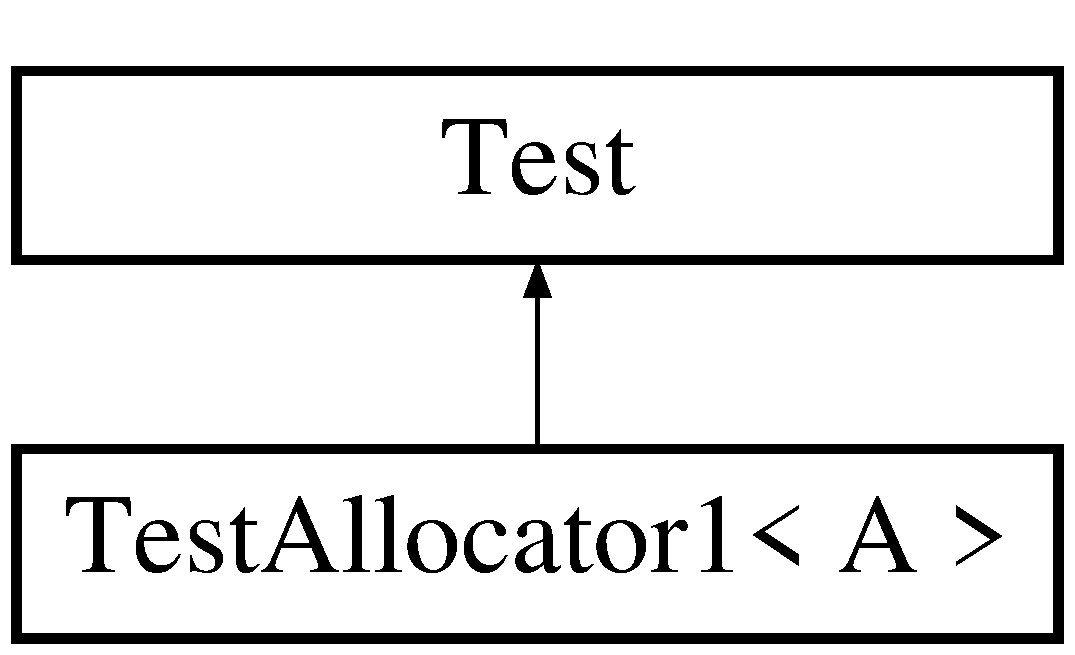
\includegraphics[height=2.000000cm]{structTestAllocator1}
\end{center}
\end{figure}
\subsection*{Public Types}
\begin{DoxyCompactItemize}
\item 
typedef A \hyperlink{structTestAllocator1_af833c587251c56fda9cc1169d40545d5}{allocator\-\_\-type}
\item 
typedef A\-::value\-\_\-type \hyperlink{structTestAllocator1_a92fce0c8423cac5757d6b1d253d646d5}{value\-\_\-type}
\item 
typedef A\-::size\-\_\-type \hyperlink{structTestAllocator1_aa8c669c72a5405cad2024cb1f2d0213d}{size\-\_\-type}
\item 
typedef A\-::pointer \hyperlink{structTestAllocator1_a2d4b518664da974c318e96f1d5fe8cf5}{pointer}
\end{DoxyCompactItemize}


\subsection{Member Typedef Documentation}
\hypertarget{structTestAllocator1_af833c587251c56fda9cc1169d40545d5}{\index{Test\-Allocator1@{Test\-Allocator1}!allocator\-\_\-type@{allocator\-\_\-type}}
\index{allocator\-\_\-type@{allocator\-\_\-type}!TestAllocator1@{Test\-Allocator1}}
\subsubsection[{allocator\-\_\-type}]{\setlength{\rightskip}{0pt plus 5cm}template$<$typename A $>$ typedef A {\bf Test\-Allocator1}$<$ A $>$\-::{\bf allocator\-\_\-type}}}\label{structTestAllocator1_af833c587251c56fda9cc1169d40545d5}
\hypertarget{structTestAllocator1_a2d4b518664da974c318e96f1d5fe8cf5}{\index{Test\-Allocator1@{Test\-Allocator1}!pointer@{pointer}}
\index{pointer@{pointer}!TestAllocator1@{Test\-Allocator1}}
\subsubsection[{pointer}]{\setlength{\rightskip}{0pt plus 5cm}template$<$typename A $>$ typedef A\-::pointer {\bf Test\-Allocator1}$<$ A $>$\-::{\bf pointer}}}\label{structTestAllocator1_a2d4b518664da974c318e96f1d5fe8cf5}
\hypertarget{structTestAllocator1_aa8c669c72a5405cad2024cb1f2d0213d}{\index{Test\-Allocator1@{Test\-Allocator1}!size\-\_\-type@{size\-\_\-type}}
\index{size\-\_\-type@{size\-\_\-type}!TestAllocator1@{Test\-Allocator1}}
\subsubsection[{size\-\_\-type}]{\setlength{\rightskip}{0pt plus 5cm}template$<$typename A $>$ typedef A\-::size\-\_\-type {\bf Test\-Allocator1}$<$ A $>$\-::{\bf size\-\_\-type}}}\label{structTestAllocator1_aa8c669c72a5405cad2024cb1f2d0213d}
\hypertarget{structTestAllocator1_a92fce0c8423cac5757d6b1d253d646d5}{\index{Test\-Allocator1@{Test\-Allocator1}!value\-\_\-type@{value\-\_\-type}}
\index{value\-\_\-type@{value\-\_\-type}!TestAllocator1@{Test\-Allocator1}}
\subsubsection[{value\-\_\-type}]{\setlength{\rightskip}{0pt plus 5cm}template$<$typename A $>$ typedef A\-::value\-\_\-type {\bf Test\-Allocator1}$<$ A $>$\-::{\bf value\-\_\-type}}}\label{structTestAllocator1_a92fce0c8423cac5757d6b1d253d646d5}


The documentation for this struct was generated from the following file\-:\begin{DoxyCompactItemize}
\item 
\hyperlink{TestAllocator_8c_09_09}{Test\-Allocator.\-c++}\end{DoxyCompactItemize}

\hypertarget{structTestAllocator3}{\section{Test\-Allocator3$<$ A $>$ Struct Template Reference}
\label{structTestAllocator3}\index{Test\-Allocator3$<$ A $>$@{Test\-Allocator3$<$ A $>$}}
}
Inheritance diagram for Test\-Allocator3$<$ A $>$\-:\begin{figure}[H]
\begin{center}
\leavevmode
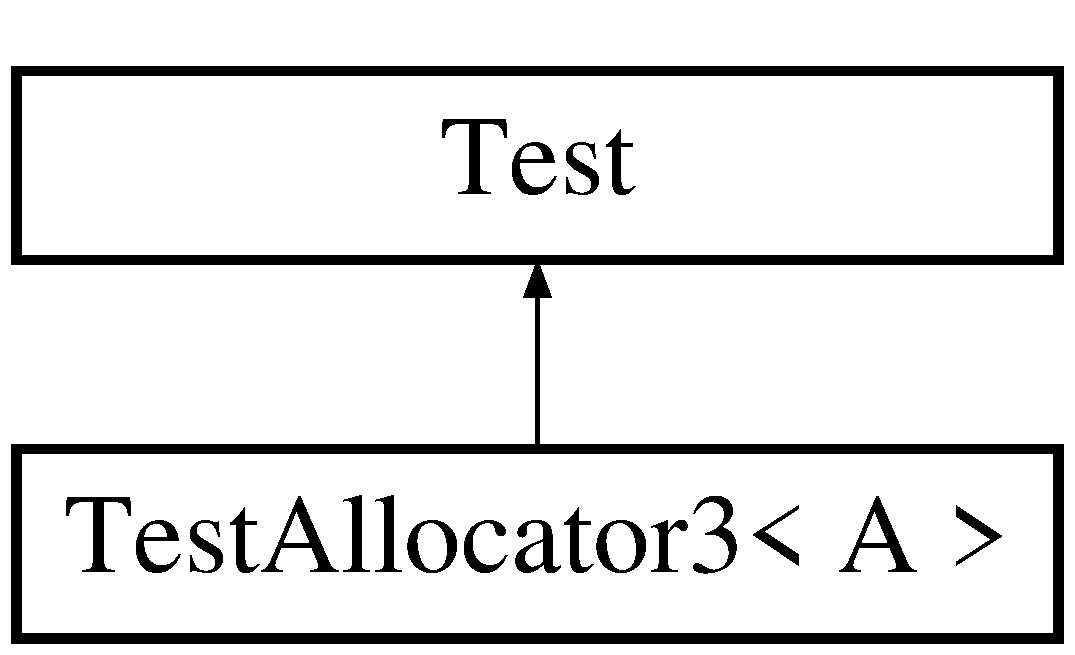
\includegraphics[height=2.000000cm]{structTestAllocator3}
\end{center}
\end{figure}
\subsection*{Public Types}
\begin{DoxyCompactItemize}
\item 
typedef A \hyperlink{structTestAllocator3_a2cbf292b14532b741aa9c2d29603cecd}{allocator\-\_\-type}
\item 
typedef A\-::value\-\_\-type \hyperlink{structTestAllocator3_ac5054dfad63609102029f3bda09f70fc}{value\-\_\-type}
\item 
typedef A\-::size\-\_\-type \hyperlink{structTestAllocator3_a123816b6d7f35344795ee12a478658d8}{size\-\_\-type}
\item 
typedef A\-::pointer \hyperlink{structTestAllocator3_a1e00e0a73b38d61279e77535325b2124}{pointer}
\end{DoxyCompactItemize}


\subsection{Member Typedef Documentation}
\hypertarget{structTestAllocator3_a2cbf292b14532b741aa9c2d29603cecd}{\index{Test\-Allocator3@{Test\-Allocator3}!allocator\-\_\-type@{allocator\-\_\-type}}
\index{allocator\-\_\-type@{allocator\-\_\-type}!TestAllocator3@{Test\-Allocator3}}
\subsubsection[{allocator\-\_\-type}]{\setlength{\rightskip}{0pt plus 5cm}template$<$typename A $>$ typedef A {\bf Test\-Allocator3}$<$ A $>$\-::{\bf allocator\-\_\-type}}}\label{structTestAllocator3_a2cbf292b14532b741aa9c2d29603cecd}
\hypertarget{structTestAllocator3_a1e00e0a73b38d61279e77535325b2124}{\index{Test\-Allocator3@{Test\-Allocator3}!pointer@{pointer}}
\index{pointer@{pointer}!TestAllocator3@{Test\-Allocator3}}
\subsubsection[{pointer}]{\setlength{\rightskip}{0pt plus 5cm}template$<$typename A $>$ typedef A\-::pointer {\bf Test\-Allocator3}$<$ A $>$\-::{\bf pointer}}}\label{structTestAllocator3_a1e00e0a73b38d61279e77535325b2124}
\hypertarget{structTestAllocator3_a123816b6d7f35344795ee12a478658d8}{\index{Test\-Allocator3@{Test\-Allocator3}!size\-\_\-type@{size\-\_\-type}}
\index{size\-\_\-type@{size\-\_\-type}!TestAllocator3@{Test\-Allocator3}}
\subsubsection[{size\-\_\-type}]{\setlength{\rightskip}{0pt plus 5cm}template$<$typename A $>$ typedef A\-::size\-\_\-type {\bf Test\-Allocator3}$<$ A $>$\-::{\bf size\-\_\-type}}}\label{structTestAllocator3_a123816b6d7f35344795ee12a478658d8}
\hypertarget{structTestAllocator3_ac5054dfad63609102029f3bda09f70fc}{\index{Test\-Allocator3@{Test\-Allocator3}!value\-\_\-type@{value\-\_\-type}}
\index{value\-\_\-type@{value\-\_\-type}!TestAllocator3@{Test\-Allocator3}}
\subsubsection[{value\-\_\-type}]{\setlength{\rightskip}{0pt plus 5cm}template$<$typename A $>$ typedef A\-::value\-\_\-type {\bf Test\-Allocator3}$<$ A $>$\-::{\bf value\-\_\-type}}}\label{structTestAllocator3_ac5054dfad63609102029f3bda09f70fc}


The documentation for this struct was generated from the following file\-:\begin{DoxyCompactItemize}
\item 
\hyperlink{TestAllocator_8c_09_09}{Test\-Allocator.\-c++}\end{DoxyCompactItemize}

\chapter{File Documentation}
\hypertarget{Allocator_8h}{\section{Allocator.\-h File Reference}
\label{Allocator_8h}\index{Allocator.\-h@{Allocator.\-h}}
}
{\ttfamily \#include $<$cassert$>$}\\*
{\ttfamily \#include $<$cstddef$>$}\\*
{\ttfamily \#include $<$new$>$}\\*
{\ttfamily \#include $<$stdexcept$>$}\\*
\subsection*{Classes}
\begin{DoxyCompactItemize}
\item 
class \hyperlink{classAllocator}{Allocator$<$ T, N $>$}
\end{DoxyCompactItemize}
\subsection*{Macros}
\begin{DoxyCompactItemize}
\item 
\#define \hyperlink{Allocator_8h_a72c133601bb43024f531278312851b2e}{S\-E\-N\-T\-I\-N\-E\-L\-\_\-\-T\-Y\-P\-E}~int
\end{DoxyCompactItemize}
\subsection*{Functions}
\begin{DoxyCompactItemize}
\item 
static int \hyperlink{Allocator_8h_a5421e33950566d606165773f704ea144}{abs\-\_\-val} (int x)
\end{DoxyCompactItemize}


\subsection{Macro Definition Documentation}
\hypertarget{Allocator_8h_a72c133601bb43024f531278312851b2e}{\index{Allocator.\-h@{Allocator.\-h}!S\-E\-N\-T\-I\-N\-E\-L\-\_\-\-T\-Y\-P\-E@{S\-E\-N\-T\-I\-N\-E\-L\-\_\-\-T\-Y\-P\-E}}
\index{S\-E\-N\-T\-I\-N\-E\-L\-\_\-\-T\-Y\-P\-E@{S\-E\-N\-T\-I\-N\-E\-L\-\_\-\-T\-Y\-P\-E}!Allocator.h@{Allocator.\-h}}
\subsubsection[{S\-E\-N\-T\-I\-N\-E\-L\-\_\-\-T\-Y\-P\-E}]{\setlength{\rightskip}{0pt plus 5cm}\#define S\-E\-N\-T\-I\-N\-E\-L\-\_\-\-T\-Y\-P\-E~int}}\label{Allocator_8h_a72c133601bb43024f531278312851b2e}


\subsection{Function Documentation}
\hypertarget{Allocator_8h_a5421e33950566d606165773f704ea144}{\index{Allocator.\-h@{Allocator.\-h}!abs\-\_\-val@{abs\-\_\-val}}
\index{abs\-\_\-val@{abs\-\_\-val}!Allocator.h@{Allocator.\-h}}
\subsubsection[{abs\-\_\-val}]{\setlength{\rightskip}{0pt plus 5cm}static int abs\-\_\-val (
\begin{DoxyParamCaption}
\item[{int}]{x}
\end{DoxyParamCaption}
)\hspace{0.3cm}{\ttfamily [static]}}}\label{Allocator_8h_a5421e33950566d606165773f704ea144}
O(1) in space O(1) in time calculates $\vert$x$\vert$ and returns the value 
\hypertarget{README_8md}{\section{R\-E\-A\-D\-M\-E.\-md File Reference}
\label{README_8md}\index{R\-E\-A\-D\-M\-E.\-md@{R\-E\-A\-D\-M\-E.\-md}}
}

\hypertarget{TestAllocator_8c_09_09}{\section{Test\-Allocator.\-c++ File Reference}
\label{TestAllocator_8c_09_09}\index{Test\-Allocator.\-c++@{Test\-Allocator.\-c++}}
}
{\ttfamily \#include $<$algorithm$>$}\\*
{\ttfamily \#include $<$memory$>$}\\*
{\ttfamily \#include \char`\"{}gtest/gtest.\-h\char`\"{}}\\*
{\ttfamily \#include \char`\"{}Allocator.\-h\char`\"{}}\\*
\subsection*{Classes}
\begin{DoxyCompactItemize}
\item 
struct \hyperlink{structTestAllocator1}{Test\-Allocator1$<$ A $>$}
\item 
struct \hyperlink{structTestAllocator3}{Test\-Allocator3$<$ A $>$}
\end{DoxyCompactItemize}
\subsection*{Typedefs}
\begin{DoxyCompactItemize}
\item 
typedef testing\-::\-Types\\*
$<$ std\-::allocator$<$ int $>$\\*
, std\-::allocator$<$ double $>$\\*
, \hyperlink{classAllocator}{Allocator}$<$ int, 100 $>$\\*
, \hyperlink{classAllocator}{Allocator}$<$ double, 100 $>$ $>$ \hyperlink{TestAllocator_8c_09_09_a13869bd8140d5f03f67a74c18b4a9483}{my\-\_\-types\-\_\-1}
\item 
typedef testing\-::\-Types\\*
$<$ \hyperlink{classAllocator}{Allocator}$<$ int, 100 $>$\\*
, \hyperlink{classAllocator}{Allocator}$<$ double, 100 $>$ $>$ \hyperlink{TestAllocator_8c_09_09_ae8c7ebc24b7c1269b8c59135bef34e20}{my\-\_\-types\-\_\-2}
\end{DoxyCompactItemize}
\subsection*{Functions}
\begin{DoxyCompactItemize}
\item 
\hyperlink{TestAllocator_8c_09_09_ac12bb00f418021d252bd2c25ece50c93}{T\-Y\-P\-E\-D\-\_\-\-T\-E\-S\-T\-\_\-\-C\-A\-S\-E} (\hyperlink{structTestAllocator1}{Test\-Allocator1}, \hyperlink{TestAllocator_8c_09_09_a13869bd8140d5f03f67a74c18b4a9483}{my\-\_\-types\-\_\-1})
\item 
\hyperlink{TestAllocator_8c_09_09_ae7f896b998cca25e9dd5fb6e0ee4eebc}{T\-Y\-P\-E\-D\-\_\-\-T\-E\-S\-T} (\hyperlink{structTestAllocator1}{Test\-Allocator1}, test\-\_\-1)
\item 
\hyperlink{TestAllocator_8c_09_09_aa2803b82f1082b0ae849ad3075c944ad}{T\-Y\-P\-E\-D\-\_\-\-T\-E\-S\-T} (\hyperlink{structTestAllocator1}{Test\-Allocator1}, test\-\_\-10)
\item 
\hyperlink{TestAllocator_8c_09_09_a204cc10f9bc1ca26b04bad4656b87671}{T\-E\-S\-T} (Test\-Allocator2, const\-\_\-index)
\item 
\hyperlink{TestAllocator_8c_09_09_a4da97a8aeec81f53d36b25e8483d51ec}{T\-E\-S\-T} (Test\-Allocator2, index)
\item 
\hyperlink{TestAllocator_8c_09_09_a2834e7174b70f38555c1dc1808e6ce3b}{T\-Y\-P\-E\-D\-\_\-\-T\-E\-S\-T\-\_\-\-C\-A\-S\-E} (\hyperlink{structTestAllocator3}{Test\-Allocator3}, \hyperlink{TestAllocator_8c_09_09_ae8c7ebc24b7c1269b8c59135bef34e20}{my\-\_\-types\-\_\-2})
\item 
\hyperlink{TestAllocator_8c_09_09_a0a98bdf8c103a8a929e22e100a185ea2}{T\-Y\-P\-E\-D\-\_\-\-T\-E\-S\-T} (\hyperlink{structTestAllocator3}{Test\-Allocator3}, test\-\_\-1)
\item 
\hyperlink{TestAllocator_8c_09_09_a8160ba0a226c52d48c08bf80c72fde03}{T\-Y\-P\-E\-D\-\_\-\-T\-E\-S\-T} (\hyperlink{structTestAllocator3}{Test\-Allocator3}, test\-\_\-10)
\item 
\hyperlink{TestAllocator_8c_09_09_a7e0f24656a410bacb1041e5c2dd07801}{T\-E\-S\-T} (Test\-Allocator\-Constructor, construct\-\_\-int)
\item 
\hyperlink{TestAllocator_8c_09_09_af0ede47de50329774cb3d71b3e640bb1}{T\-E\-S\-T} (Test\-Allocator\-Constructor, construct\-\_\-exception)
\item 
\hyperlink{TestAllocator_8c_09_09_aa9ecbe57010651a59974079b34ec6ac7}{T\-E\-S\-T} (Test\-Allocator\-Constructor, construct\-\_\-double)
\item 
\hyperlink{TestAllocator_8c_09_09_aa030c002a0a4ec39efd41ec32a8a5f7c}{T\-E\-S\-T} (Test\-Allocator\-Valid, valid1)
\item 
\hyperlink{TestAllocator_8c_09_09_a1eb51325a4526d8fc5dfea45f8f41c06}{T\-E\-S\-T} (Test\-Allocator\-Valid, valid2)
\item 
\hyperlink{TestAllocator_8c_09_09_a2b4a5601315a39925c4b11733c76d13a}{T\-E\-S\-T} (Test\-Allocator\-Valid, valid3)
\item 
\hyperlink{TestAllocator_8c_09_09_a88fa712af9be1fe8601173aaad0d17a9}{T\-E\-S\-T} (Test\-Allocator\-Allocate, allocate1)
\item 
\hyperlink{TestAllocator_8c_09_09_a03ba40dc8d564df913b7819e88cbe6ab}{T\-E\-S\-T} (Test\-Allocator\-Allocate, allocate2)
\item 
\hyperlink{TestAllocator_8c_09_09_a9f9aefe29328486d62b3bec1b5c2bf16}{T\-E\-S\-T} (Test\-Allocator\-Allocate, allocate3)
\item 
\hyperlink{TestAllocator_8c_09_09_ab8b6a4d933c13070c1c57f3a907997f2}{T\-E\-S\-T} (Test\-Allocator\-Allocate, allocate\-\_\-toomuch)
\item 
\hyperlink{TestAllocator_8c_09_09_a7e55640d98d2c17ec4e4c03ce3b06828}{T\-E\-S\-T} (Test\-Allocator\-Allocate, allocate\-\_\-negative)
\item 
\hyperlink{TestAllocator_8c_09_09_a77b90ff75b91cecaba99f039f838b047}{T\-E\-S\-T} (Test\-Allocator\-Allocate, allocate\-\_\-zero)
\item 
\hyperlink{TestAllocator_8c_09_09_ab255499288b1ba1445e8762228aedbe5}{T\-E\-S\-T} (Test\-Allocator\-Deallocate, deallocate1)
\item 
\hyperlink{TestAllocator_8c_09_09_ac12a713e609cda2a46b4d78b858ee907}{T\-E\-S\-T} (Test\-Allocator\-Deallocate, deallocate2)
\item 
\hyperlink{TestAllocator_8c_09_09_afc15ba460c09b299d4a9eab06f5b1602}{T\-E\-S\-T} (Test\-Allocator\-Deallocate, deallocate3)
\item 
\hyperlink{TestAllocator_8c_09_09_ad21682e7c75eb2e95b5a7443db79df71}{T\-E\-S\-T} (Test\-Allocator\-Deallocate, exception)
\end{DoxyCompactItemize}


\subsection{Typedef Documentation}
\hypertarget{TestAllocator_8c_09_09_a13869bd8140d5f03f67a74c18b4a9483}{\index{Test\-Allocator.\-c++@{Test\-Allocator.\-c++}!my\-\_\-types\-\_\-1@{my\-\_\-types\-\_\-1}}
\index{my\-\_\-types\-\_\-1@{my\-\_\-types\-\_\-1}!TestAllocator.c++@{Test\-Allocator.\-c++}}
\subsubsection[{my\-\_\-types\-\_\-1}]{\setlength{\rightskip}{0pt plus 5cm}typedef testing\-::\-Types$<$ std\-::allocator$<$int$>$, std\-::allocator$<$double$>$, {\bf Allocator}$<$int, 100$>$, {\bf Allocator}$<$double, 100$>$ $>$ {\bf my\-\_\-types\-\_\-1}}}\label{TestAllocator_8c_09_09_a13869bd8140d5f03f67a74c18b4a9483}
\hypertarget{TestAllocator_8c_09_09_ae8c7ebc24b7c1269b8c59135bef34e20}{\index{Test\-Allocator.\-c++@{Test\-Allocator.\-c++}!my\-\_\-types\-\_\-2@{my\-\_\-types\-\_\-2}}
\index{my\-\_\-types\-\_\-2@{my\-\_\-types\-\_\-2}!TestAllocator.c++@{Test\-Allocator.\-c++}}
\subsubsection[{my\-\_\-types\-\_\-2}]{\setlength{\rightskip}{0pt plus 5cm}typedef testing\-::\-Types$<$ {\bf Allocator}$<$int, 100$>$, {\bf Allocator}$<$double, 100$>$ $>$ {\bf my\-\_\-types\-\_\-2}}}\label{TestAllocator_8c_09_09_ae8c7ebc24b7c1269b8c59135bef34e20}


\subsection{Function Documentation}
\hypertarget{TestAllocator_8c_09_09_a204cc10f9bc1ca26b04bad4656b87671}{\index{Test\-Allocator.\-c++@{Test\-Allocator.\-c++}!T\-E\-S\-T@{T\-E\-S\-T}}
\index{T\-E\-S\-T@{T\-E\-S\-T}!TestAllocator.c++@{Test\-Allocator.\-c++}}
\subsubsection[{T\-E\-S\-T}]{\setlength{\rightskip}{0pt plus 5cm}T\-E\-S\-T (
\begin{DoxyParamCaption}
\item[{Test\-Allocator2}]{, }
\item[{const\-\_\-index}]{}
\end{DoxyParamCaption}
)}}\label{TestAllocator_8c_09_09_a204cc10f9bc1ca26b04bad4656b87671}
\hypertarget{TestAllocator_8c_09_09_a4da97a8aeec81f53d36b25e8483d51ec}{\index{Test\-Allocator.\-c++@{Test\-Allocator.\-c++}!T\-E\-S\-T@{T\-E\-S\-T}}
\index{T\-E\-S\-T@{T\-E\-S\-T}!TestAllocator.c++@{Test\-Allocator.\-c++}}
\subsubsection[{T\-E\-S\-T}]{\setlength{\rightskip}{0pt plus 5cm}T\-E\-S\-T (
\begin{DoxyParamCaption}
\item[{Test\-Allocator2}]{, }
\item[{index}]{}
\end{DoxyParamCaption}
)}}\label{TestAllocator_8c_09_09_a4da97a8aeec81f53d36b25e8483d51ec}
\hypertarget{TestAllocator_8c_09_09_a7e0f24656a410bacb1041e5c2dd07801}{\index{Test\-Allocator.\-c++@{Test\-Allocator.\-c++}!T\-E\-S\-T@{T\-E\-S\-T}}
\index{T\-E\-S\-T@{T\-E\-S\-T}!TestAllocator.c++@{Test\-Allocator.\-c++}}
\subsubsection[{T\-E\-S\-T}]{\setlength{\rightskip}{0pt plus 5cm}T\-E\-S\-T (
\begin{DoxyParamCaption}
\item[{Test\-Allocator\-Constructor}]{, }
\item[{construct\-\_\-int}]{}
\end{DoxyParamCaption}
)}}\label{TestAllocator_8c_09_09_a7e0f24656a410bacb1041e5c2dd07801}
\hypertarget{TestAllocator_8c_09_09_af0ede47de50329774cb3d71b3e640bb1}{\index{Test\-Allocator.\-c++@{Test\-Allocator.\-c++}!T\-E\-S\-T@{T\-E\-S\-T}}
\index{T\-E\-S\-T@{T\-E\-S\-T}!TestAllocator.c++@{Test\-Allocator.\-c++}}
\subsubsection[{T\-E\-S\-T}]{\setlength{\rightskip}{0pt plus 5cm}T\-E\-S\-T (
\begin{DoxyParamCaption}
\item[{Test\-Allocator\-Constructor}]{, }
\item[{construct\-\_\-exception}]{}
\end{DoxyParamCaption}
)}}\label{TestAllocator_8c_09_09_af0ede47de50329774cb3d71b3e640bb1}
\hypertarget{TestAllocator_8c_09_09_aa9ecbe57010651a59974079b34ec6ac7}{\index{Test\-Allocator.\-c++@{Test\-Allocator.\-c++}!T\-E\-S\-T@{T\-E\-S\-T}}
\index{T\-E\-S\-T@{T\-E\-S\-T}!TestAllocator.c++@{Test\-Allocator.\-c++}}
\subsubsection[{T\-E\-S\-T}]{\setlength{\rightskip}{0pt plus 5cm}T\-E\-S\-T (
\begin{DoxyParamCaption}
\item[{Test\-Allocator\-Constructor}]{, }
\item[{construct\-\_\-double}]{}
\end{DoxyParamCaption}
)}}\label{TestAllocator_8c_09_09_aa9ecbe57010651a59974079b34ec6ac7}
\hypertarget{TestAllocator_8c_09_09_aa030c002a0a4ec39efd41ec32a8a5f7c}{\index{Test\-Allocator.\-c++@{Test\-Allocator.\-c++}!T\-E\-S\-T@{T\-E\-S\-T}}
\index{T\-E\-S\-T@{T\-E\-S\-T}!TestAllocator.c++@{Test\-Allocator.\-c++}}
\subsubsection[{T\-E\-S\-T}]{\setlength{\rightskip}{0pt plus 5cm}T\-E\-S\-T (
\begin{DoxyParamCaption}
\item[{Test\-Allocator\-Valid}]{, }
\item[{valid1}]{}
\end{DoxyParamCaption}
)}}\label{TestAllocator_8c_09_09_aa030c002a0a4ec39efd41ec32a8a5f7c}
\hypertarget{TestAllocator_8c_09_09_a1eb51325a4526d8fc5dfea45f8f41c06}{\index{Test\-Allocator.\-c++@{Test\-Allocator.\-c++}!T\-E\-S\-T@{T\-E\-S\-T}}
\index{T\-E\-S\-T@{T\-E\-S\-T}!TestAllocator.c++@{Test\-Allocator.\-c++}}
\subsubsection[{T\-E\-S\-T}]{\setlength{\rightskip}{0pt plus 5cm}T\-E\-S\-T (
\begin{DoxyParamCaption}
\item[{Test\-Allocator\-Valid}]{, }
\item[{valid2}]{}
\end{DoxyParamCaption}
)}}\label{TestAllocator_8c_09_09_a1eb51325a4526d8fc5dfea45f8f41c06}
\hypertarget{TestAllocator_8c_09_09_a2b4a5601315a39925c4b11733c76d13a}{\index{Test\-Allocator.\-c++@{Test\-Allocator.\-c++}!T\-E\-S\-T@{T\-E\-S\-T}}
\index{T\-E\-S\-T@{T\-E\-S\-T}!TestAllocator.c++@{Test\-Allocator.\-c++}}
\subsubsection[{T\-E\-S\-T}]{\setlength{\rightskip}{0pt plus 5cm}T\-E\-S\-T (
\begin{DoxyParamCaption}
\item[{Test\-Allocator\-Valid}]{, }
\item[{valid3}]{}
\end{DoxyParamCaption}
)}}\label{TestAllocator_8c_09_09_a2b4a5601315a39925c4b11733c76d13a}
\hypertarget{TestAllocator_8c_09_09_a88fa712af9be1fe8601173aaad0d17a9}{\index{Test\-Allocator.\-c++@{Test\-Allocator.\-c++}!T\-E\-S\-T@{T\-E\-S\-T}}
\index{T\-E\-S\-T@{T\-E\-S\-T}!TestAllocator.c++@{Test\-Allocator.\-c++}}
\subsubsection[{T\-E\-S\-T}]{\setlength{\rightskip}{0pt plus 5cm}T\-E\-S\-T (
\begin{DoxyParamCaption}
\item[{Test\-Allocator\-Allocate}]{, }
\item[{allocate1}]{}
\end{DoxyParamCaption}
)}}\label{TestAllocator_8c_09_09_a88fa712af9be1fe8601173aaad0d17a9}
\hypertarget{TestAllocator_8c_09_09_a03ba40dc8d564df913b7819e88cbe6ab}{\index{Test\-Allocator.\-c++@{Test\-Allocator.\-c++}!T\-E\-S\-T@{T\-E\-S\-T}}
\index{T\-E\-S\-T@{T\-E\-S\-T}!TestAllocator.c++@{Test\-Allocator.\-c++}}
\subsubsection[{T\-E\-S\-T}]{\setlength{\rightskip}{0pt plus 5cm}T\-E\-S\-T (
\begin{DoxyParamCaption}
\item[{Test\-Allocator\-Allocate}]{, }
\item[{allocate2}]{}
\end{DoxyParamCaption}
)}}\label{TestAllocator_8c_09_09_a03ba40dc8d564df913b7819e88cbe6ab}
\hypertarget{TestAllocator_8c_09_09_a9f9aefe29328486d62b3bec1b5c2bf16}{\index{Test\-Allocator.\-c++@{Test\-Allocator.\-c++}!T\-E\-S\-T@{T\-E\-S\-T}}
\index{T\-E\-S\-T@{T\-E\-S\-T}!TestAllocator.c++@{Test\-Allocator.\-c++}}
\subsubsection[{T\-E\-S\-T}]{\setlength{\rightskip}{0pt plus 5cm}T\-E\-S\-T (
\begin{DoxyParamCaption}
\item[{Test\-Allocator\-Allocate}]{, }
\item[{allocate3}]{}
\end{DoxyParamCaption}
)}}\label{TestAllocator_8c_09_09_a9f9aefe29328486d62b3bec1b5c2bf16}
\hypertarget{TestAllocator_8c_09_09_ab8b6a4d933c13070c1c57f3a907997f2}{\index{Test\-Allocator.\-c++@{Test\-Allocator.\-c++}!T\-E\-S\-T@{T\-E\-S\-T}}
\index{T\-E\-S\-T@{T\-E\-S\-T}!TestAllocator.c++@{Test\-Allocator.\-c++}}
\subsubsection[{T\-E\-S\-T}]{\setlength{\rightskip}{0pt plus 5cm}T\-E\-S\-T (
\begin{DoxyParamCaption}
\item[{Test\-Allocator\-Allocate}]{, }
\item[{allocate\-\_\-toomuch}]{}
\end{DoxyParamCaption}
)}}\label{TestAllocator_8c_09_09_ab8b6a4d933c13070c1c57f3a907997f2}
\hypertarget{TestAllocator_8c_09_09_a7e55640d98d2c17ec4e4c03ce3b06828}{\index{Test\-Allocator.\-c++@{Test\-Allocator.\-c++}!T\-E\-S\-T@{T\-E\-S\-T}}
\index{T\-E\-S\-T@{T\-E\-S\-T}!TestAllocator.c++@{Test\-Allocator.\-c++}}
\subsubsection[{T\-E\-S\-T}]{\setlength{\rightskip}{0pt plus 5cm}T\-E\-S\-T (
\begin{DoxyParamCaption}
\item[{Test\-Allocator\-Allocate}]{, }
\item[{allocate\-\_\-negative}]{}
\end{DoxyParamCaption}
)}}\label{TestAllocator_8c_09_09_a7e55640d98d2c17ec4e4c03ce3b06828}
\hypertarget{TestAllocator_8c_09_09_a77b90ff75b91cecaba99f039f838b047}{\index{Test\-Allocator.\-c++@{Test\-Allocator.\-c++}!T\-E\-S\-T@{T\-E\-S\-T}}
\index{T\-E\-S\-T@{T\-E\-S\-T}!TestAllocator.c++@{Test\-Allocator.\-c++}}
\subsubsection[{T\-E\-S\-T}]{\setlength{\rightskip}{0pt plus 5cm}T\-E\-S\-T (
\begin{DoxyParamCaption}
\item[{Test\-Allocator\-Allocate}]{, }
\item[{allocate\-\_\-zero}]{}
\end{DoxyParamCaption}
)}}\label{TestAllocator_8c_09_09_a77b90ff75b91cecaba99f039f838b047}
\hypertarget{TestAllocator_8c_09_09_ab255499288b1ba1445e8762228aedbe5}{\index{Test\-Allocator.\-c++@{Test\-Allocator.\-c++}!T\-E\-S\-T@{T\-E\-S\-T}}
\index{T\-E\-S\-T@{T\-E\-S\-T}!TestAllocator.c++@{Test\-Allocator.\-c++}}
\subsubsection[{T\-E\-S\-T}]{\setlength{\rightskip}{0pt plus 5cm}T\-E\-S\-T (
\begin{DoxyParamCaption}
\item[{Test\-Allocator\-Deallocate}]{, }
\item[{deallocate1}]{}
\end{DoxyParamCaption}
)}}\label{TestAllocator_8c_09_09_ab255499288b1ba1445e8762228aedbe5}
\hypertarget{TestAllocator_8c_09_09_ac12a713e609cda2a46b4d78b858ee907}{\index{Test\-Allocator.\-c++@{Test\-Allocator.\-c++}!T\-E\-S\-T@{T\-E\-S\-T}}
\index{T\-E\-S\-T@{T\-E\-S\-T}!TestAllocator.c++@{Test\-Allocator.\-c++}}
\subsubsection[{T\-E\-S\-T}]{\setlength{\rightskip}{0pt plus 5cm}T\-E\-S\-T (
\begin{DoxyParamCaption}
\item[{Test\-Allocator\-Deallocate}]{, }
\item[{deallocate2}]{}
\end{DoxyParamCaption}
)}}\label{TestAllocator_8c_09_09_ac12a713e609cda2a46b4d78b858ee907}
\hypertarget{TestAllocator_8c_09_09_afc15ba460c09b299d4a9eab06f5b1602}{\index{Test\-Allocator.\-c++@{Test\-Allocator.\-c++}!T\-E\-S\-T@{T\-E\-S\-T}}
\index{T\-E\-S\-T@{T\-E\-S\-T}!TestAllocator.c++@{Test\-Allocator.\-c++}}
\subsubsection[{T\-E\-S\-T}]{\setlength{\rightskip}{0pt plus 5cm}T\-E\-S\-T (
\begin{DoxyParamCaption}
\item[{Test\-Allocator\-Deallocate}]{, }
\item[{deallocate3}]{}
\end{DoxyParamCaption}
)}}\label{TestAllocator_8c_09_09_afc15ba460c09b299d4a9eab06f5b1602}
\hypertarget{TestAllocator_8c_09_09_ad21682e7c75eb2e95b5a7443db79df71}{\index{Test\-Allocator.\-c++@{Test\-Allocator.\-c++}!T\-E\-S\-T@{T\-E\-S\-T}}
\index{T\-E\-S\-T@{T\-E\-S\-T}!TestAllocator.c++@{Test\-Allocator.\-c++}}
\subsubsection[{T\-E\-S\-T}]{\setlength{\rightskip}{0pt plus 5cm}T\-E\-S\-T (
\begin{DoxyParamCaption}
\item[{Test\-Allocator\-Deallocate}]{, }
\item[{exception}]{}
\end{DoxyParamCaption}
)}}\label{TestAllocator_8c_09_09_ad21682e7c75eb2e95b5a7443db79df71}
\hypertarget{TestAllocator_8c_09_09_ae7f896b998cca25e9dd5fb6e0ee4eebc}{\index{Test\-Allocator.\-c++@{Test\-Allocator.\-c++}!T\-Y\-P\-E\-D\-\_\-\-T\-E\-S\-T@{T\-Y\-P\-E\-D\-\_\-\-T\-E\-S\-T}}
\index{T\-Y\-P\-E\-D\-\_\-\-T\-E\-S\-T@{T\-Y\-P\-E\-D\-\_\-\-T\-E\-S\-T}!TestAllocator.c++@{Test\-Allocator.\-c++}}
\subsubsection[{T\-Y\-P\-E\-D\-\_\-\-T\-E\-S\-T}]{\setlength{\rightskip}{0pt plus 5cm}T\-Y\-P\-E\-D\-\_\-\-T\-E\-S\-T (
\begin{DoxyParamCaption}
\item[{{\bf Test\-Allocator1}}]{, }
\item[{test\-\_\-1}]{}
\end{DoxyParamCaption}
)}}\label{TestAllocator_8c_09_09_ae7f896b998cca25e9dd5fb6e0ee4eebc}
\hypertarget{TestAllocator_8c_09_09_aa2803b82f1082b0ae849ad3075c944ad}{\index{Test\-Allocator.\-c++@{Test\-Allocator.\-c++}!T\-Y\-P\-E\-D\-\_\-\-T\-E\-S\-T@{T\-Y\-P\-E\-D\-\_\-\-T\-E\-S\-T}}
\index{T\-Y\-P\-E\-D\-\_\-\-T\-E\-S\-T@{T\-Y\-P\-E\-D\-\_\-\-T\-E\-S\-T}!TestAllocator.c++@{Test\-Allocator.\-c++}}
\subsubsection[{T\-Y\-P\-E\-D\-\_\-\-T\-E\-S\-T}]{\setlength{\rightskip}{0pt plus 5cm}T\-Y\-P\-E\-D\-\_\-\-T\-E\-S\-T (
\begin{DoxyParamCaption}
\item[{{\bf Test\-Allocator1}}]{, }
\item[{test\-\_\-10}]{}
\end{DoxyParamCaption}
)}}\label{TestAllocator_8c_09_09_aa2803b82f1082b0ae849ad3075c944ad}
\hypertarget{TestAllocator_8c_09_09_a0a98bdf8c103a8a929e22e100a185ea2}{\index{Test\-Allocator.\-c++@{Test\-Allocator.\-c++}!T\-Y\-P\-E\-D\-\_\-\-T\-E\-S\-T@{T\-Y\-P\-E\-D\-\_\-\-T\-E\-S\-T}}
\index{T\-Y\-P\-E\-D\-\_\-\-T\-E\-S\-T@{T\-Y\-P\-E\-D\-\_\-\-T\-E\-S\-T}!TestAllocator.c++@{Test\-Allocator.\-c++}}
\subsubsection[{T\-Y\-P\-E\-D\-\_\-\-T\-E\-S\-T}]{\setlength{\rightskip}{0pt plus 5cm}T\-Y\-P\-E\-D\-\_\-\-T\-E\-S\-T (
\begin{DoxyParamCaption}
\item[{{\bf Test\-Allocator3}}]{, }
\item[{test\-\_\-1}]{}
\end{DoxyParamCaption}
)}}\label{TestAllocator_8c_09_09_a0a98bdf8c103a8a929e22e100a185ea2}
\hypertarget{TestAllocator_8c_09_09_a8160ba0a226c52d48c08bf80c72fde03}{\index{Test\-Allocator.\-c++@{Test\-Allocator.\-c++}!T\-Y\-P\-E\-D\-\_\-\-T\-E\-S\-T@{T\-Y\-P\-E\-D\-\_\-\-T\-E\-S\-T}}
\index{T\-Y\-P\-E\-D\-\_\-\-T\-E\-S\-T@{T\-Y\-P\-E\-D\-\_\-\-T\-E\-S\-T}!TestAllocator.c++@{Test\-Allocator.\-c++}}
\subsubsection[{T\-Y\-P\-E\-D\-\_\-\-T\-E\-S\-T}]{\setlength{\rightskip}{0pt plus 5cm}T\-Y\-P\-E\-D\-\_\-\-T\-E\-S\-T (
\begin{DoxyParamCaption}
\item[{{\bf Test\-Allocator3}}]{, }
\item[{test\-\_\-10}]{}
\end{DoxyParamCaption}
)}}\label{TestAllocator_8c_09_09_a8160ba0a226c52d48c08bf80c72fde03}
\hypertarget{TestAllocator_8c_09_09_ac12bb00f418021d252bd2c25ece50c93}{\index{Test\-Allocator.\-c++@{Test\-Allocator.\-c++}!T\-Y\-P\-E\-D\-\_\-\-T\-E\-S\-T\-\_\-\-C\-A\-S\-E@{T\-Y\-P\-E\-D\-\_\-\-T\-E\-S\-T\-\_\-\-C\-A\-S\-E}}
\index{T\-Y\-P\-E\-D\-\_\-\-T\-E\-S\-T\-\_\-\-C\-A\-S\-E@{T\-Y\-P\-E\-D\-\_\-\-T\-E\-S\-T\-\_\-\-C\-A\-S\-E}!TestAllocator.c++@{Test\-Allocator.\-c++}}
\subsubsection[{T\-Y\-P\-E\-D\-\_\-\-T\-E\-S\-T\-\_\-\-C\-A\-S\-E}]{\setlength{\rightskip}{0pt plus 5cm}T\-Y\-P\-E\-D\-\_\-\-T\-E\-S\-T\-\_\-\-C\-A\-S\-E (
\begin{DoxyParamCaption}
\item[{{\bf Test\-Allocator1}}]{, }
\item[{{\bf my\-\_\-types\-\_\-1}}]{}
\end{DoxyParamCaption}
)}}\label{TestAllocator_8c_09_09_ac12bb00f418021d252bd2c25ece50c93}
\hypertarget{TestAllocator_8c_09_09_a2834e7174b70f38555c1dc1808e6ce3b}{\index{Test\-Allocator.\-c++@{Test\-Allocator.\-c++}!T\-Y\-P\-E\-D\-\_\-\-T\-E\-S\-T\-\_\-\-C\-A\-S\-E@{T\-Y\-P\-E\-D\-\_\-\-T\-E\-S\-T\-\_\-\-C\-A\-S\-E}}
\index{T\-Y\-P\-E\-D\-\_\-\-T\-E\-S\-T\-\_\-\-C\-A\-S\-E@{T\-Y\-P\-E\-D\-\_\-\-T\-E\-S\-T\-\_\-\-C\-A\-S\-E}!TestAllocator.c++@{Test\-Allocator.\-c++}}
\subsubsection[{T\-Y\-P\-E\-D\-\_\-\-T\-E\-S\-T\-\_\-\-C\-A\-S\-E}]{\setlength{\rightskip}{0pt plus 5cm}T\-Y\-P\-E\-D\-\_\-\-T\-E\-S\-T\-\_\-\-C\-A\-S\-E (
\begin{DoxyParamCaption}
\item[{{\bf Test\-Allocator3}}]{, }
\item[{{\bf my\-\_\-types\-\_\-2}}]{}
\end{DoxyParamCaption}
)}}\label{TestAllocator_8c_09_09_a2834e7174b70f38555c1dc1808e6ce3b}

%--- End generated contents ---

% Index
\newpage
\phantomsection
\addcontentsline{toc}{chapter}{Index}
\printindex

\end{document}
